\section{UDP measurements}\label{sec_udp_mes}

\subsection*{Purpose:}

To determine the maximum frequency that can be used with the UDP protocol. To do so, we will measure the round time trip delay and jitter and look at those values as a function of the delay used in the sending loop.

\subsection*{Test equipment:}

The sbRIO 9636 is connected to a computer running Ubuntu 14.04 LTS via an Ethernet cable of 1 gpbs. The computer runs the ROS nodes that are used for the project, thus it communicates with both the Geomagic Touch and the sbRIO and it sends random setpoints to the sbRIO. The sbRIO uses the entire code of the project.

\subsection*{Procedure:}

\begin{enumerate}
	\item The sbRIO is started and connected to the computer.
	\item The ROS node is started.
	\item tshark is started.% using this command: $tshark -i 1 -f udp -a duration:20 -w ~/wireshark_capture$
	\item Once the Wireshark recording is done the ROS node is stopped.
	\item The log files are retrieved to be analyzed using Matlab and Wireshark.
\end{enumerate}
Those steps are repeated for both the serial and parallel case for the following settings: 10 ms, 2 ms and 0 ms.


\subsection*{Measuring data:}

\begin{center}
	$\begin{tabular}{c|ccccc}
		\text{Delay} & \text{Sending frequency (Hz)} & \text{Receiving frequency (Hz)} & \text{Average delay (ms)} & \text{Jitter} & \text{Error rate (\%)}\\
		\hline
		10ms & 86 & 86 & 1.8 & 2.7 & 0 \\
		2ms & 447 & 447 & 2.1 & 3.5 & 1.2E-4 \\
		0ms & 981 & 981 & 1.4 & 2.7 & 5.1E-5 \\
	\end{tabular}$
	\captionof{table}{UDP}
\end{center}

\begin{figure}[H]

    \centering

    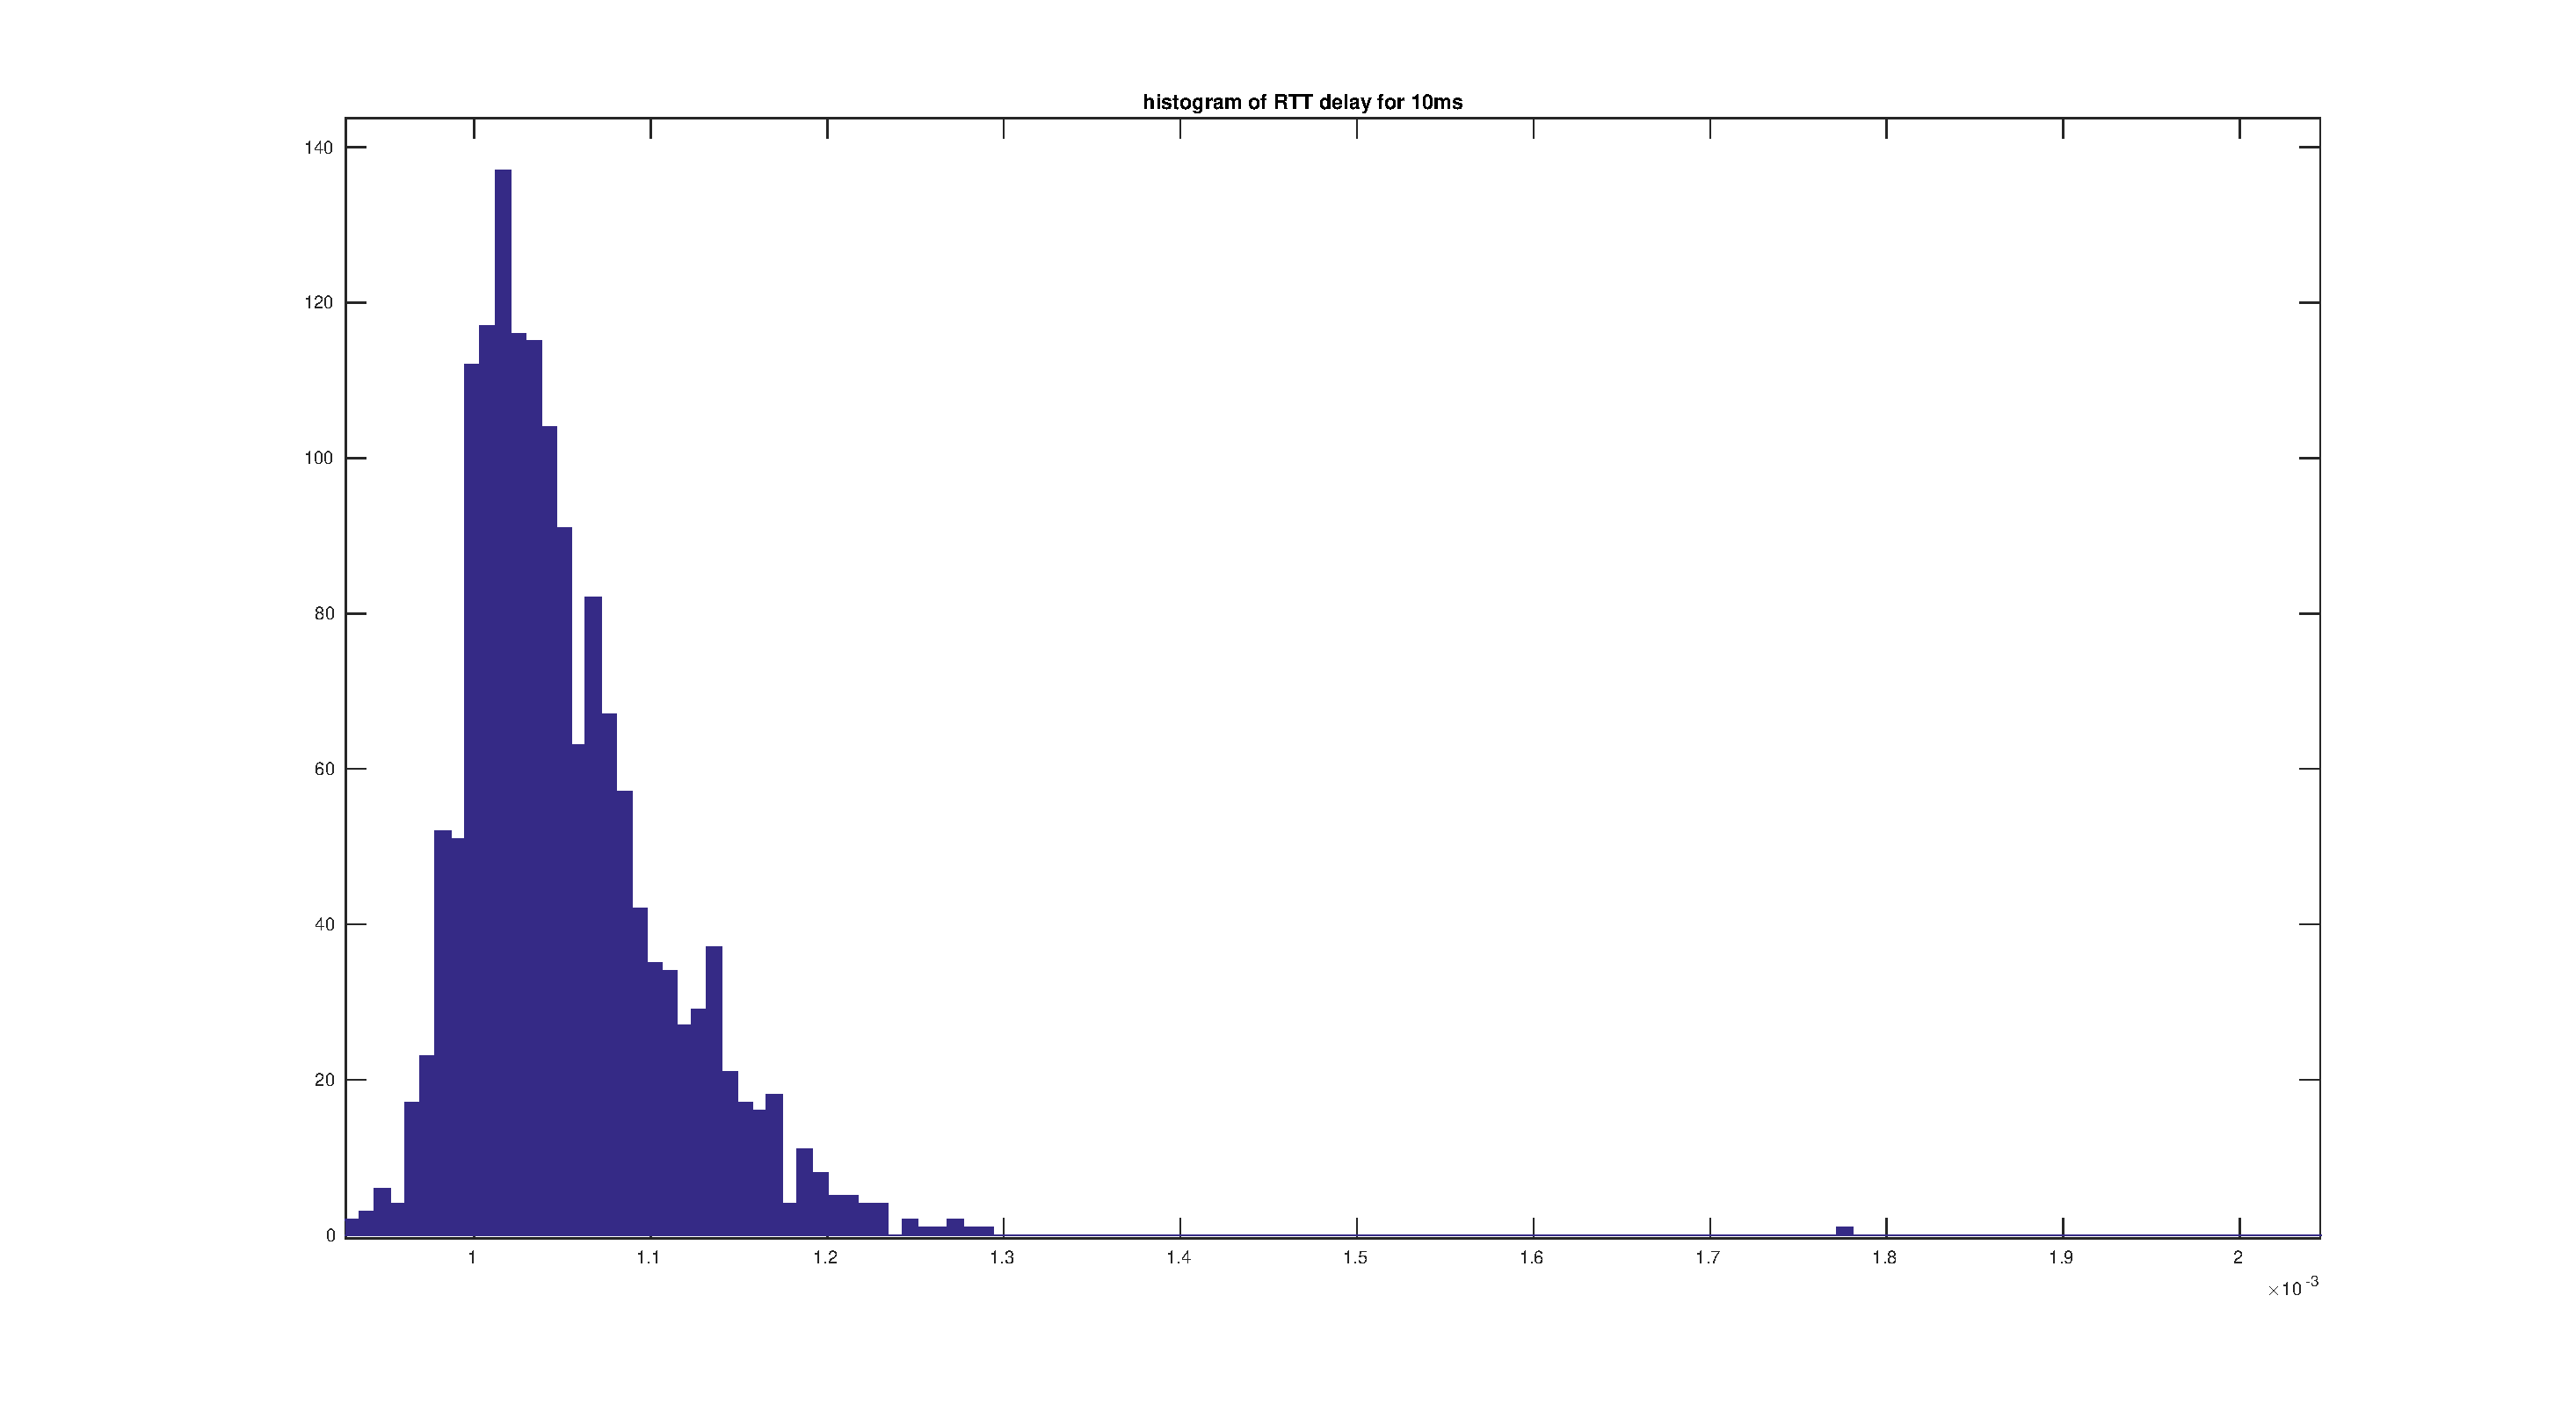
\includegraphics[width=\linewidth]{10ms}

    \caption{10ms}

\end{figure} 

\begin{figure}[H]

    \centering

    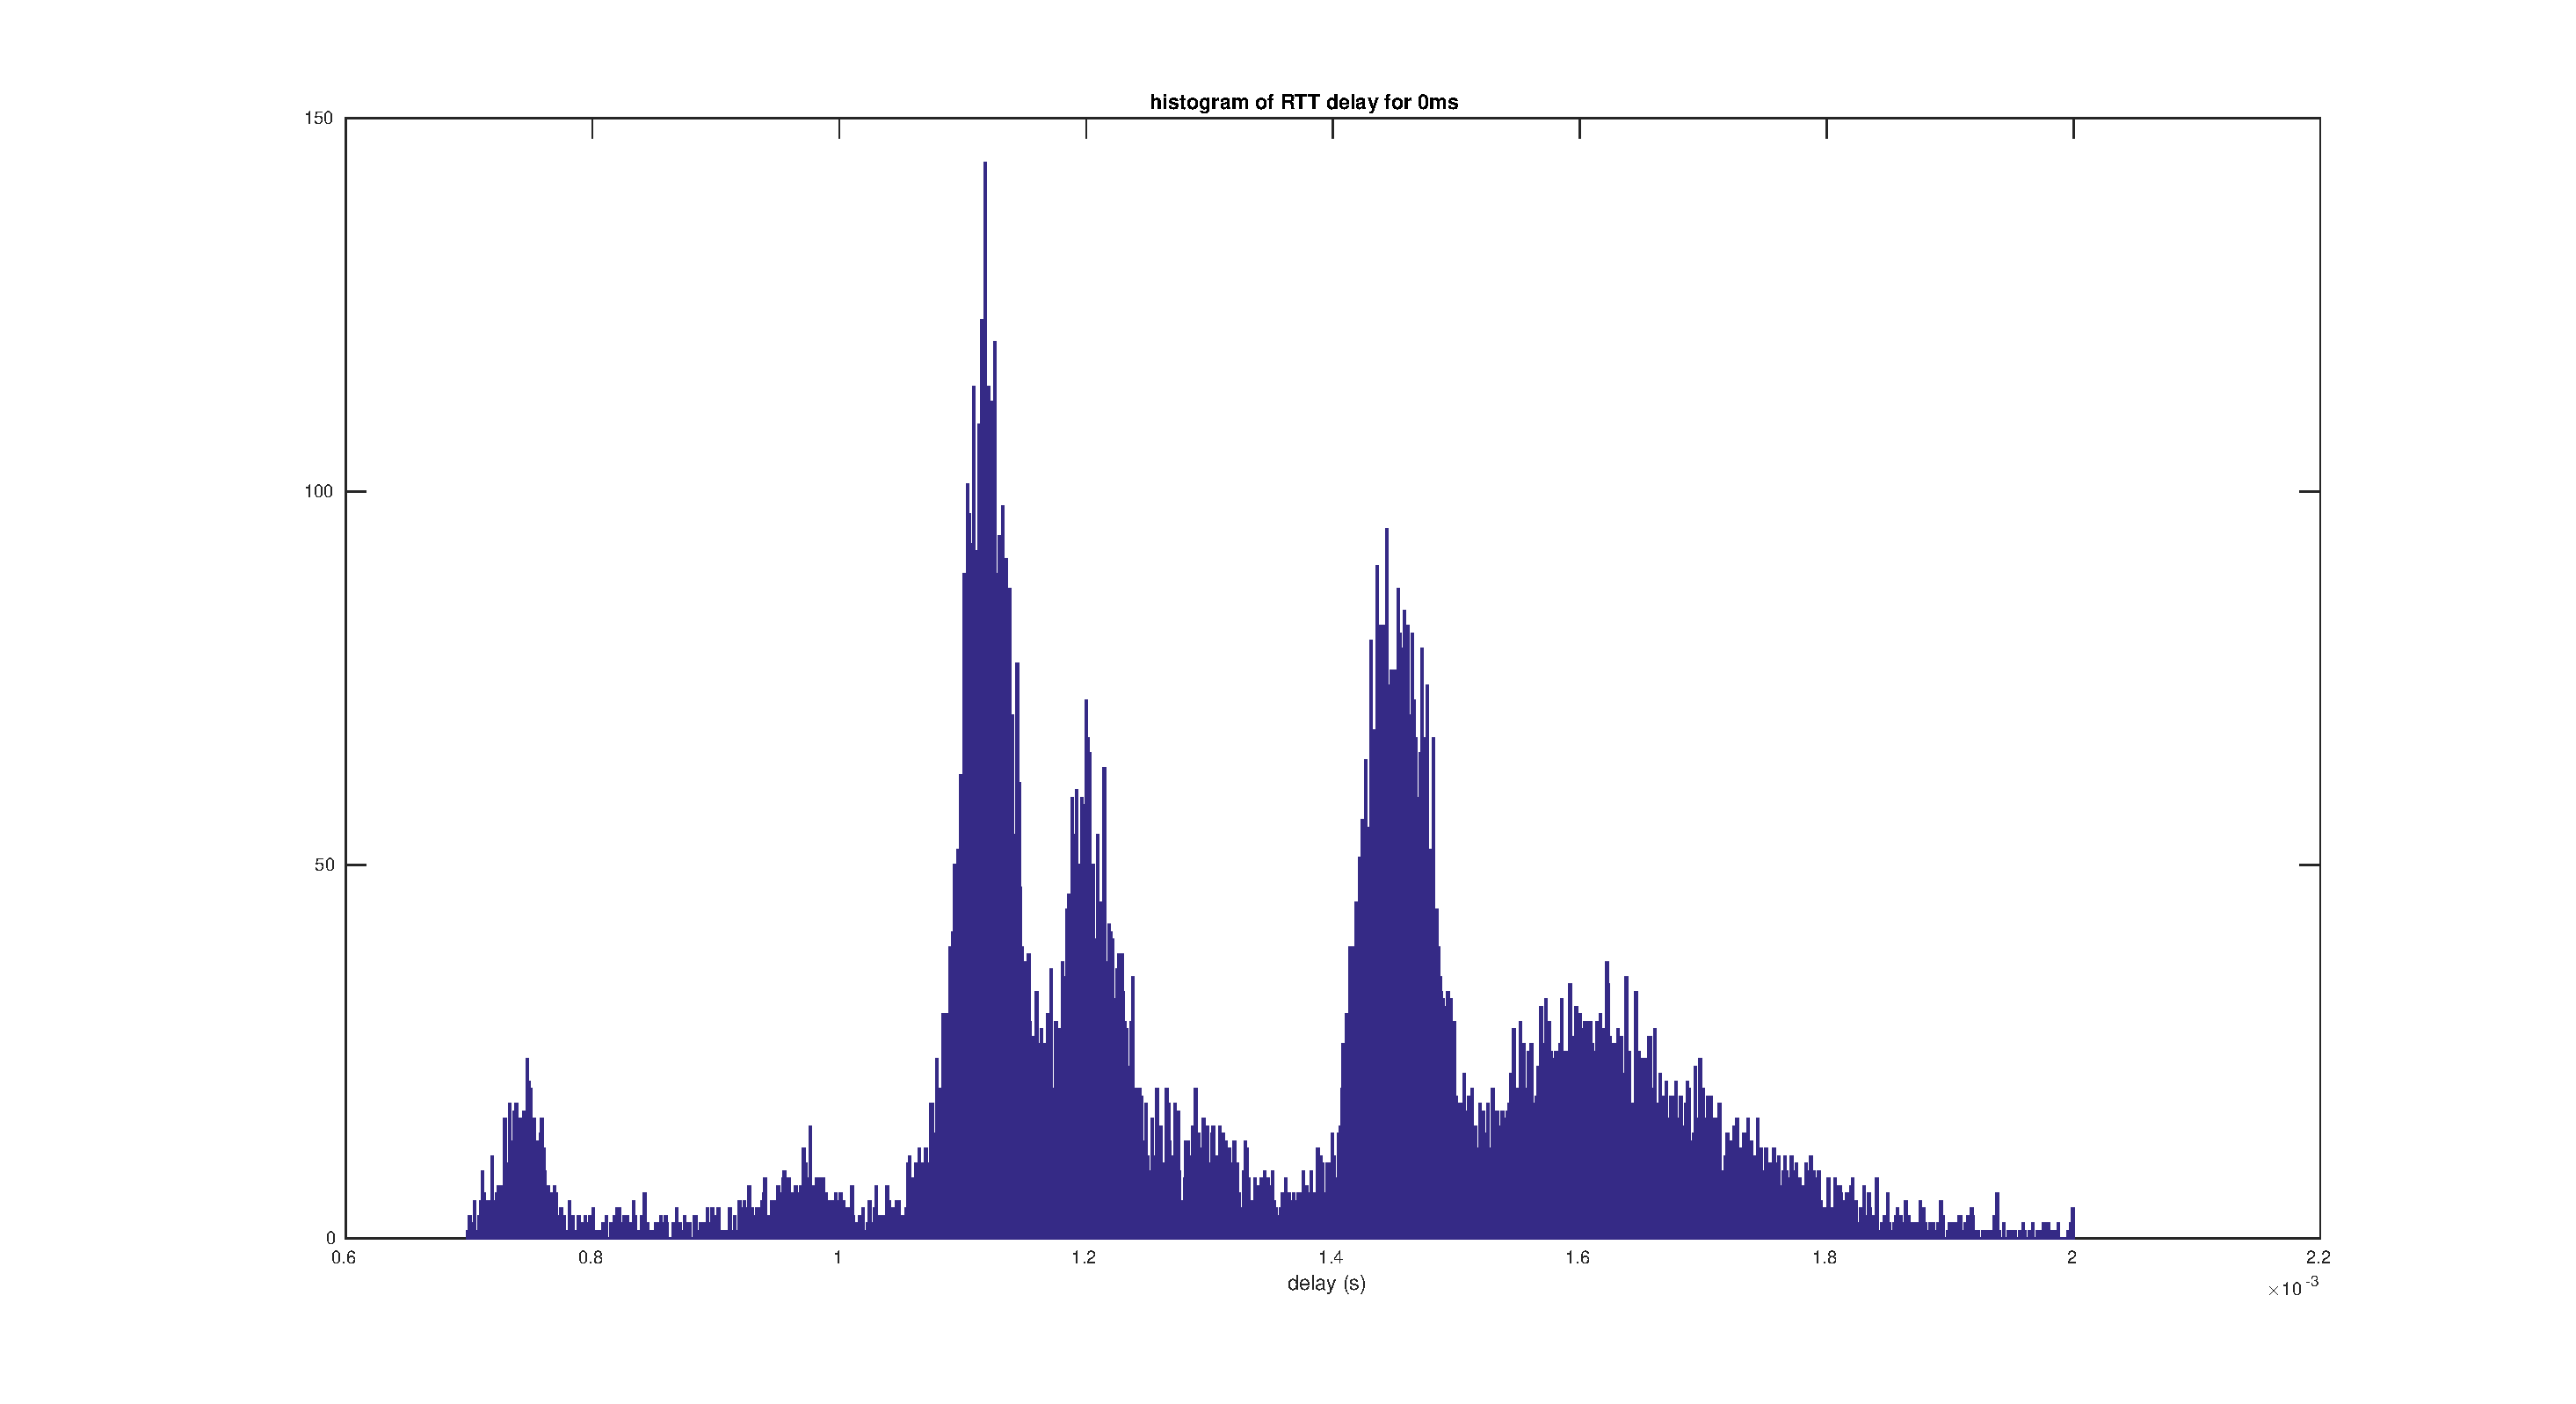
\includegraphics[width=\linewidth]{0ms}

    \caption{0ms}

\end{figure} 

\todo{remake graph and table with more data set}



\subsection*{Results:}

As the frequency of the communication increases, the delay becomes more and more sensitive to the disturbances caused by the preemption of other processes on the computer and as such the behavior of the system will become unpredictable. 


\subsection*{Uncertainties of measurement:}

??

\subsection*{Conclusion:}

Hopefully UDP is faster.